\chapter{Implementation Plan}


\section{Schedule(Gantt Chart)}
	
	\begin{figure}[h]
	 \centering
	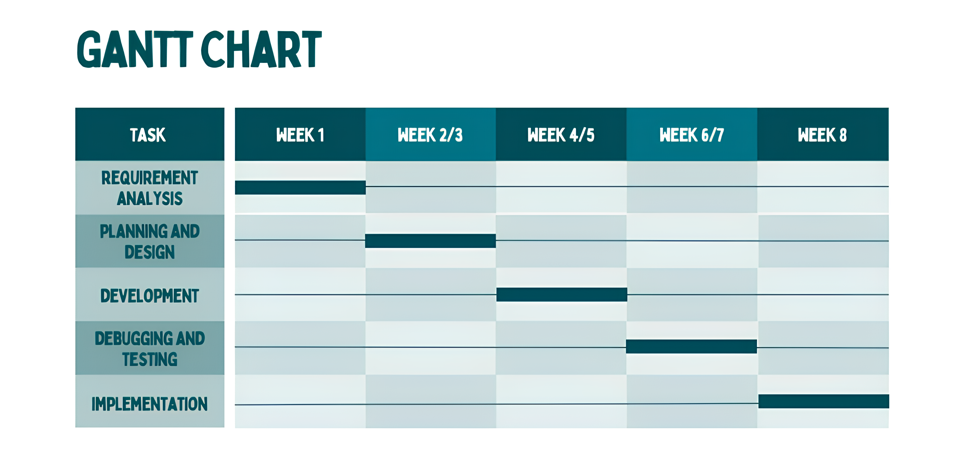
\includegraphics[scale=1]{images/Gyant_chart.png}
	\caption{ Gantt Chart}
	
	\end{figure}
	
	\pagebreak
	\section{Hardware and Software Requirements}
	\subsection{Software Requirements}
 	\subsubsection{Python and Deep Learning}
We will be using Python as our programming language for this project. Python is a high-level general-purpose computer programming language often used to build websites and software, automate tasks, and conduct data analysis. It is simple, free, easy to use and highly compatible language consisting of a lot of libraries as well as built-in data structures. Having better library ecosystem, better visualization options, platform independence ,and it’s well known simplicity, consistency and flexibility, Python has proven itself to be one of the best picks for Artificial Intelligence and Machine Learning. Machine learning is a branch of Artificial Intelligence, where we start with an image and extract it’s salient features. Then we create a model that describes or predicts the object on the basis of those features. On the other hand, for Deep Learning, we skip the manual step of extracting the features from the object and directly feed the images into a Deep Learning Algorithm, which then predicts the object. Deep Learning can be used to eliminate the limitations of Machine Learning since it makes it easier to handle complex problems as well as helps us predict through huge amount of data with ease too. Thus, Deep learning is a subset of machine learning which provides the ability to machine to perform human-like tasks without human involvement. It provides the ability to an AI agent to mimic the human brain. Deep learning can use both supervised and unsupervised learning to train an AI agent. Here we will try to utilize technique of Deep Learning and concepts of computerized neural networks using Python for the completion for this project. It serves as the primary programming language for  lip reading project, providing a flexible and easy-to-read syntax.
\break
\subsubsection{OpenCV}
OpenCV is an open-source computer vision library that provides a wide range of tools and functions for image and video processing. In our lip-reading project, we use OpenCV to capture and process video frames, apply image preprocessing techniques (such as resizing, filtering, and normalization), and extract relevant features from lip movements such as color or shape information. It also converts the preprocessed frames into a format suitable for input to a PyTorch model.
\break
\pagebreak
\subsubsection{PyTorch}
PyTorch is a deep learning framework that is widely used for building and training neural networks. In the context of lip reading, PyTorch can be employed to create and train deep learning models, such as convolutional neural networks (CNNs) or recurrent neural networks (RNNs). These models can learn to recognize patterns in lip movements and extract meaningful information for lip reading.
\break
\subsubsection{Matplotlib}
Matplotlib is a plotting library for Python that allows  to create a variety of static, animated, and interactive visualizations. In  lip reading project, Matplotlib can be used for visualizing different aspects of  data and results. For example, we use it to plot training/validation curves, display video frames with overlaid predictions, or create graphs to illustrate the performance of the lip reading model. The Matplotlib is used to visualize the training/validation loss curves during model training.By combining these tools, we can create a comprehensive lip reading system that leverage computer vision, deep learning and visualization to understand and interpret lip movements from video data.

\break
\section{Functional and Non-Functional Requirements}
\subsection{Functional Requirements}
\begin{enumerate}
\item \textbf{Pre-processing :}
\begin{itemize}
\item Identify and track the face in the video sequence
\item Extract the region of interest (ROI) containing the mouth.
\item Normalize the ROI with respect to size and orientation. 

\end{itemize}
\item  \textbf{Feature Extraction:}
\begin{itemize}
\item Extract relevant features from the mouth region, such as lip shape, contour, and movement dynamics. 
\item Utilize deep learning models (e.g., Convolutional Neural Networks) to achieve accurate feature extraction.


\end{itemize}
\item \textbf{Phoneme Recognition}
\begin{itemize}
\item Based on the extracted features, classify the visual information into corresponding phonemes.
\item Employ deep learning models trained on large lip-to-phoneme datasets.


\end{itemize}
\item \textbf{Sentence Formation}
\begin{itemize}
\item Combine the recognized phonemes into complete words and sentences using language models. 
\item Consider contextual information to resolve ambiguities and improve accuracy.


\end{itemize}


\end{enumerate}
\subsection{Non-Functional Requirements}
\begin{enumerate}
\item \textbf{Accuracy}
\begin{itemize}
\item The system should achieve a high level of accuracy in translating lip movements to phonemes and subsequently to words and sentences.  
\item Specify a target accuracy percentage based on existing benchmarks or project goals. 


\end{itemize}
\item \textbf{Real-time performance}
\begin{itemize}
\item The system should process and translate visual information with minimal latency, ideally in real-time.  
\item Define an acceptable delay threshold for lip-to-text conversion. 


\end{itemize}
\item \textbf{Robustness}
\begin{itemize}
\item The system should perform well under varying conditions, including different lighting, facial expressions, and speakers.   
\item Specify the range of scenarios you want the system to handle efficiently. 


\end{itemize}
\item \textbf{User Interface}
\begin{itemize}
\item The system should have a user-friendly interface for capturing video, displaying results, and interacting with the system.   
\item The system should have a user-friendly interface for capturing video, displaying results, and interacting with the system. 


\end{itemize}

\item \textbf{Resource Efficiency}
\begin{itemize}
\item The system should be able to run efficiently on available hardware resources, without excessive memory or processing power requirements.    
\item Optimize the model and algorithms to minimize resource utilization without compromising accuracy.


\end{itemize}

\end{enumerate}

